% ****** Start of file apssamp.tex ******
%
%   This file is part of the APS files in the REVTeX 4.1 distribution.
%   Version 4.1r of REVTeX, August 2010
%
%   Copyright (c) 2009, 2010 The American Physical Society.
%
%   See the REVTeX 4 README file for restrictions and more information.
%
% TeX'ing this file requires that you have AMS-LaTeX 2.0 installed
% as well as the rest of the prerequisites for REVTeX 4.1
%
% See the REVTeX 4 README file
% It also requires running BibTeX. The commands are as follows:
%
%  1)  latex apssamp.tex
%  2)  bibtex apssamp
%  3)  latex apssamp.tex
%  4)  latex apssamp.tex
%
\documentclass[%
 reprint,
superscriptaddress,
%groupedaddress,
%unsortedaddress,
%runinaddress,
%frontmatterverbose,
%preprint,
%showpacs,preprintnumbers,
%nofootinbib,
%nobibnotes,
%bibnotes,
 amsmath,amssymb,
 aps,
%pra,
%prb,
%rmp,
%prstab,
%prstper,
%floatfix,
]{revtex4-1}

\usepackage{graphicx}% Include figure files
\usepackage{dcolumn}% Align table columns on decimal point
\usepackage{bm}% bold math
\usepackage{hyperref}% add hypertext capabilities
\usepackage[mathlines]{lineno}% Enable numbering of text and display math
\usepackage{siunitx}
\usepackage{amssymb}
%\linenumbers\relax % Commence numbering lines

%\usepackage[showframe,%Uncomment any one of the following lines to test
%%scale=0.7, marginratio={1:1, 2:3}, ignoreall,% default settings
%%text={7in,10in},centering,
%%margin=1.5in,
%%total={6.5in,8.75in}, top=1.2in, left=0.9in, includefoot,
%%height=10in,a5paper,hmargin={3cm,0.8in},
%]{geometry}

\newcommand{\R}{\mathbb{R}}

\begin{document}

\preprint{APS/123-QED}

\title{An Investigation of the Stefan-Boltzmann Law}% Force line breaks with \\

\author{Thomas Malthouse}



\maketitle

\subsection{Data and Error Analysis}

\subsubsection{High-Temperature Lab}


Table \ref{hightemp-data} shows the data collected for this experiment, as well as associated measurement errors. The measured voltage and current values were used to calculate the resistance of the lamp using Ohm's Law,
\begin{equation}\label{ohms-law}
    R = \frac{V}{I}.
\end{equation}

These resistance values were then expressed as a ratio compared to the ambient temperature, and used to find the temperature of the lamp at each voltage, using the interpolation function defined in the associated Mathematica notebook. The calculated resistances and temperatures, as well as associated errors, are shown in table \ref{ht-calcs}. By the Stefan-Boltzmann Law,
\begin{equation}
    V(T) \approx aT^4
\end{equation}
the lamp temperature and detector voltage are logarithmically related to each other, where
\begin{equation}
    \log V = C + n\log T
\end{equation}
and $n$ should be equal to four. Plotting $\log(T)$ against $\log(V_{\text{det}})$ results in figure \ref{HT-graph}. This fit gives an exponent of $n=3.1\pm0.12$, inconsistent with the expected value of 4. The graph also has a noticeable curve, indicating that the model was not correct for the data, or that the data was not collected properly. One possible source of systematic error is inaccuracies in the tungsten temperature-resistance correlation function or errors in collecting the data. The lower-temperature terms may also have been affected by the dropping of the temperature offset, which only becomes negligible at higher temperatures. The steeper slope at higher temperatures also indicates that dropping the lower temperatures could result in a slope closer to the expected value.

\subsubsection{Low-Temperature Lab}

Table \ref{LT-data} shows the data collected for the low-temperature experiment and relevant errors. The resistance values correspond to a temperature, a relation given by the \texttt{correlation3[R]} function defined in the Mathematica notebook. Applying this function gives the results found in table \ref{calc-temps-lt}.

The Stefan-Boltzmann law predicts that the temperature and detector voltage are related to each other by the equation
\begin{equation}\label{blibbity}
    V = A + BT^4
\end{equation}
where $A$ and $B$ are constants. Fitting such a model to this data results a graph resembling figure \ref{ltgraph} and resulting in $A = -5.11$ and $B = 6.78\times10^{-10}$.

Since the detector is calibrated to read a voltage of $\SI{0}{\volt}$ at room temperature, these constants can also be used to calculate a value for ambient temperature that can be compared to the measured value. Letting $V=0$ and rearranging equation \ref{blibbity} gives
\begin{equation*}
    T_0 = \left(-\frac{A}{B}\right)^{1/4} = \left(\frac{5.11}{6.78\times10^{-10}}\right)^{1/4} = \SI[separate-uncertainty = true]{294 (1)}{\kelvin}
\end{equation*}
This is a very reasonable room temperature and in line with expectations. Although the room was assumed to be $\SI{30}{\celsius} = \SI{303}{\kelvin}$, this value was never measured and is probably on the warm side. There were no significant sources of error in this experiment, and the model fit the data with a very high degree of accuracy ($R^2 = 0.99972$).


\begin{table}[b]
    \begin{tabular}{cccccc}
        \hline\hline
        $V$ (lamp) & $\Delta V$ (lamp) & $I$ & $\Delta I$ & $mV$ (detector) & $\Delta mV$ error \\  \hline
        0.0 & 0.005 & 0.0 & 0.01 & 0.01 & 0.005 \\
        0.5 & 0.005 & 0.46 & 0.02 & 0.11 & 0.015 \\
        1.0 & 0.001 & 0.571 & 0.01 & 0.16 & 0.05 \\
        1.5 & 0.001 & 0.653 & 0.01 & 0.264 & 0.005 \\
        2.0 & 0.001 & 0.729 & 0.01 & 0.423 & 0.005 \\
        2.5 & 0.001 & 0.800 & 0.01 & 0.605 & 0.008 \\
        3.0 & 0.005 & 0.868 & 0.01 & 0.834 & 0.005 \\
        3.5 & 0.001 & 0.932 & 0.01 & 1.1 & 0.01 \\
        4.0 & 0.001 & 0.994 & 0.005 & 1.43 & 0.005 \\
        4.5 & 0.001 & 1.050 & 0.005 & 1.76 & 0.005 \\
        5.0 & 0.001 & 1.107 & 0.005 & 2.11 & 0.005 \\
        5.5 & 0.001 & 1.161 & 0.005 & 2.50 & 0.005 \\
        6.0 & 0.001 & 1.214 & 0.005 & 2.89 & 0.005 \\
        6.5 & 0.001 & 1.263 & 0.005 & 3.34 & 0.005 \\
        7.0 & 0.001 & 1.211 & 0.005 & 3.83 & 0.005 \\
        7.5 & 0.001 & 1.358 & 0.005 & 4.31 & 0.005 \\
        8.0 & 0.005 & 1.403 & 0.005 & 4.8 & 0.01 \\ \hline \hline
    \end{tabular}
    \caption{Measurements for the voltage and current flowing through the lamp, and the voltage measurements from the detector.}
    \label{hightemp-data}
\end{table}

\begin{table}
\begin{tabular}{ccccc}
    \hline \hline
$V$ & $R/R_{300}$ & $\Delta R/R_{300}$ & $T$ & $\Delta T$ \\\hline
0.0 & 1.00 & 0.00 & 300 & 0 \\
0.5 & 1.85 & 0.08 & 497 & 18 \\
1.0 & 2.99 & 0.05 & 727 & 10 \\
1.5 & 3.92 & 0.06 & 908 & 11 \\
2.0 & 4.68 & 0.06 & 1050 & 12 \\
2.5 & 5.33 & 0.07 & 1172 & 13 \\
3.0 & 5.90 & 0.07 & 1276 & 12 \\
3.5 & 6.41 & 0.07 & 1369 & 12 \\
4.0 & 6.87 & 0.03 & 1451 & 6 \\
4.5 & 7.31 & 0.03 & 1531 & 6 \\
5.0 & 7.71 & 0.03 & 1600 & 6 \\
5.5 & 8.08 & 0.03 & 1666 & 6 \\
6.0 & 8.43 & 0.03 & 1727 & 6 \\
6.5 & 8.78 & 0.03 & 1787 & 6 \\
7.0 & 9.86 & 0.04 & 1972 & 7 \\
7.5 & 9.42 & 0.03 & 1897 & 6 \\
8.0 & 9.73 & 0.04 & 1949 & 6 \\ \hline \hline
\end{tabular}
    \caption{Calculated values}
    \label{ht-calcs}
\end{table}

\begin{figure}
    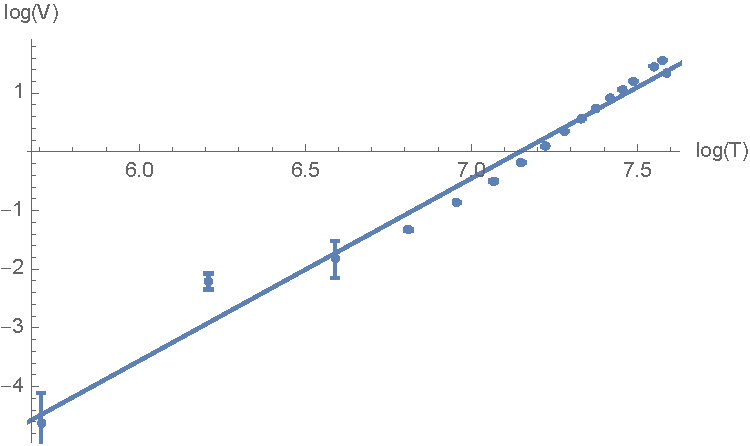
\includegraphics[width=0.4\textwidth]{floats/hightemp-graph}
    \caption{The plot of $\log(V)$ as a function of $\log(T)$. The equation of the fit curve is
    $
        \log(V) = (3.1\pm0.12) \log(T) - (22.2022\pm0.86).
    $
    Note the clear curve in the data and the ouliers at the bottom of the range.
    }
    \label{HT-graph}
\end{figure}

\begin{table}
    \begin{tabular}{ccccc}
        \hline \hline
        Target ($\si{\celsius}$) & $R (\si{\ohm}) $ & $\Delta R$ & $V_{\text{det}}$ & $\Delta V_{\text{det}}$ \\ \hline
        30 & 79400 & 200 & 0.66 & 0.005 \\
        40 & 51000 & 200 & 1.48 & 0.005 \\
        50 & 33500 & 200 & 2.20 & 0.01 \\
        60 & 22600 & 100 & 3.33 & 0.005 \\
        70 & 15500 & 100 & 4.20 & 0.01 \\
        80 & 10800 & 100 & 5.44 & 0.005 \\
        90 & 7700 & 100 & 6.70 & 0.005 \\
        100 & 5600 & 100 & 8.04 & 0.005 \\
        110 & 4070 & 30 & 9.53 & 0.005 \\
        120 & 2950 & 50 & 11.30 & 0.005 \\ \hline \hline
    \end{tabular}
    \caption{The measured results for the low-temperature lab, as well as associated errors. Note that the temperatures listed here are just target temperatures, and more accurate values will be derived from the resistance values in a later step.}
    \label{LT-data}
\end{table}

\begin{table}
    \begin{tabular}{cc} \hline \hline
        Target temp. ($\si{\celsius}$) & Actual temp. ($\si{\kelvin}$) \\ \hline
            30 & 303.15 \\
            40 & 313.15 \\
            50 & 323.15 \\
            60 & 333.15 \\
            70 & 343.15 \\
            80 & 353.15 \\
            90 & 363.15 \\
            100 & 373.15 \\
            110 & 383.25 \\
            120 & 394.09 \\ \hline \hline
    \end{tabular}
    \caption{The actual temperatures (in degrees Kelvin), and their associated target temperature (in degrees Celsius).}
    \label{calc-temps-lt}

\end{table}

\begin{figure}
    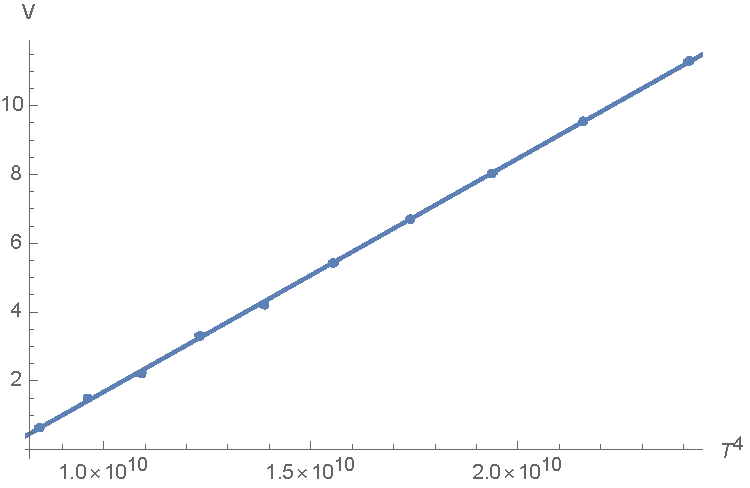
\includegraphics[width=0.4\textwidth]{floats/lowtemp-graph}
    \caption{This graph shows the relation between $T^4$ and $V_{\text{det}}$. The model has an equation of $V = (6.78\pm0.04)\times10^{-10} T - (5.1\pm0.06)$, and an $\R^2$ value of $0.99972$---indicating that the model is a very good fit for the data.}
    \label{ltgraph}
\end{figure}

\end{document}
%
% ****** End of file apssamp.tex ******
